\section{E-MOS Analytical Model}\label{sec:analytic}

With the detailed analysis and reasoning out the anamloies 
of existing power governors in the previous section, we now present our 
E-MOS (Efficient Energy Management Policies in OS) analytic model
which mainly relies on the principle of application-aware energy management. 
We believe that OS providing more freedom to user-space for energy
management is beneficial, since user-space has more relavant information about applications
and their behavior. 
Figure~\ref{fig:emos-model} \textcolor{red}{(a)} depicts the overview
of our E-MOS model.


\begin{figure}[h]
  \begin{center}
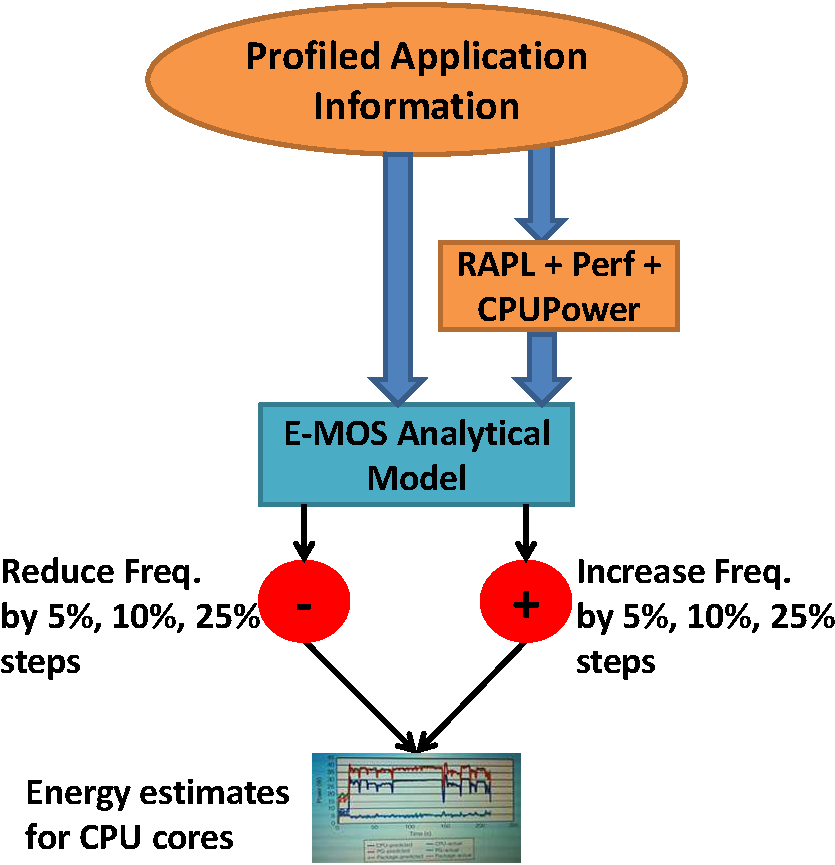
\includegraphics[width=\linewidth]{figs/EMOS-new-crop.pdf}
  \end{center}
  \vspace{-0.1in}
  \caption{a) E-MOS model; b) Frequency setting in User-space governor}
	\label{fig:emos-model}
\end{figure}





\begin{table}[h]
\footnotesize
\def\arraystretch{0.52}
\setlength{\tabcolsep}{.15em}
\center
\begin{tabular}{cccc} \toprule
Application & Objective & CPU Freq. & DRAM Freq.  \\ \midrule
Compute & Energy & Maintain\textbackslash{Increase} & Decrease \\
Compute & Performance & Increase & Maintain \\
Cache  & Energy &  Decrease & Decrease \\ 
Cache  & Performance &  Maintain & Increase \\ 
Memory & Energy & Decrease & Maintain\textbackslash{Increase} \\
Memory & Performance & Maintain & Increase \\ \midrule
\end{tabular}
\caption{E-MOS Policies Decision Table}\label{tbl:emos-dec}
\end{table}

\begin{figure}[h]
  \begin{center}
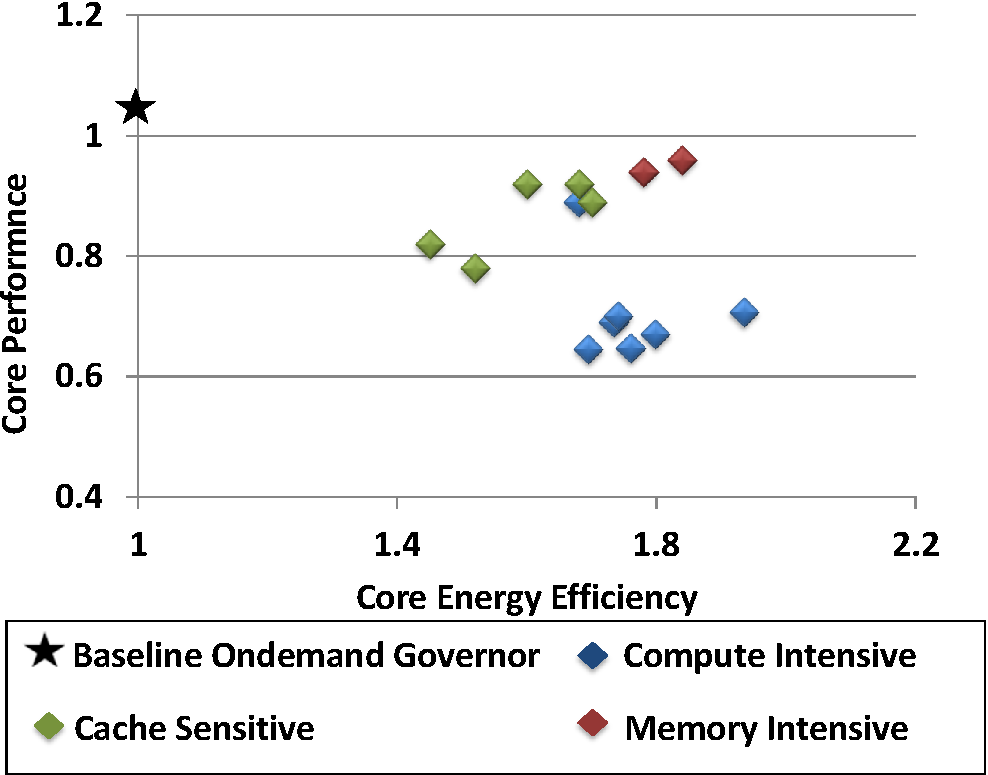
\includegraphics[width=\linewidth]{figs/ana-reduce-crop.pdf}
  \end{center}
  \vspace{-0.1in}
  \caption{Energy estimnates from E-MOS when freq. reduced by 30\% (600Mhz)}
	\label{fig:reduce-freq}
\end{figure}


\begin{figure}[h]
  \begin{center}
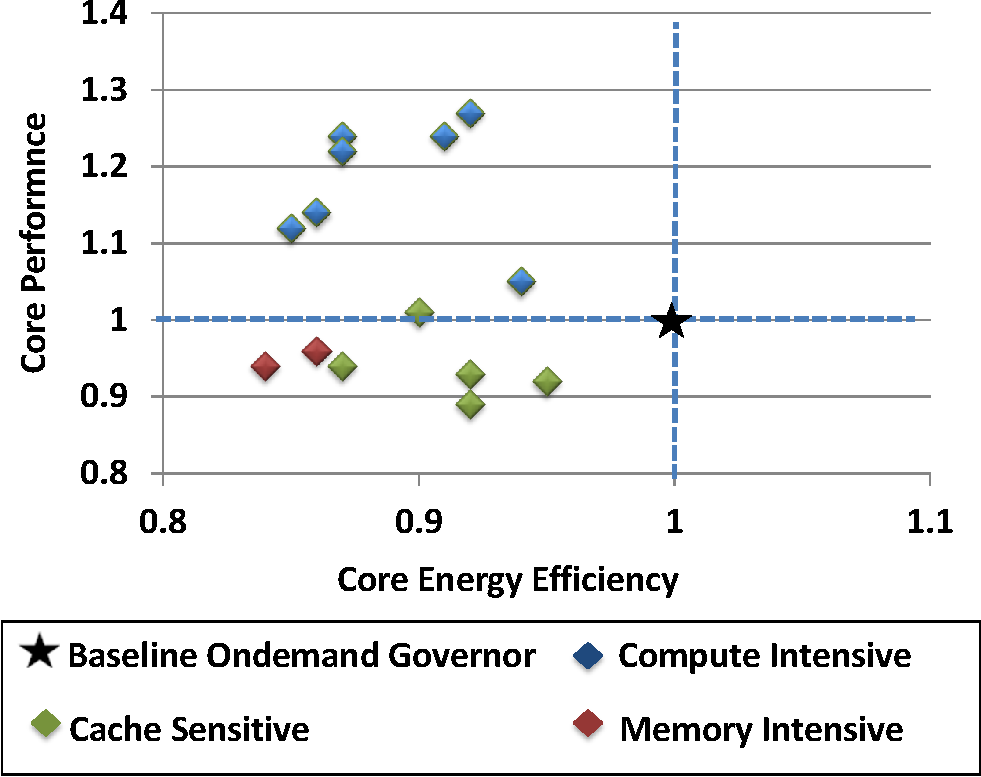
\includegraphics[width=\linewidth]{figs/ana-increase-crop.pdf}
  \end{center}
  \vspace{-0.1in}
  \caption{Energy estimnates from E-MOS when freq. increased by 30\% (600Mhz)}
	\label{fig:increase-freq}
\end{figure}

